



%%%%%%%%%%%%%%%%%%%%%%%%%%%%%
\chapter{Raisonnement par récurrence}
%%%%%%%%%%%%%%%%%%%%%%%%%%%%%


Soit $A(k)$ une assertion dépendant d'un paramètre $k$ (qui peut être un entier naturel ou relatif, un réel, en fait n'importe quel objet mathématique... mettons que le paramètre $k$ appartienne à l'ensemble $E$). Démontrer que $A(k)$ est vraie \underline{quelque soit le paramètre $k$ (dans son ensemble de définition)} est en général difficile. Le schéma de preuve est le suivant:
\emph{\begin{quote}
Soit $k \in E$. Montrons que l'assertion $A(k)$ est vraie.\\
(...ici,  preuve de $A(k)$...)\\
Donc $A(k)$ est vraie.\\
(Conclusion) Le paramètre $k$ ayant été pris arbitrairement dans l'ensemble $E$, on a bien montré que \og pour tout $k\in E$,  $A(k)$ est vraie.\fg
\end{quote}}

La difficulté est qu'il faut montrer l'assertion $A(k)$ sans rien savoir sur le paramètre $k$ (c'est justement ça qui entraîne que l'assertion est vraie pour tous les paramètres $k$ et pas juste un paramètre particulier).

Lorsque le paramètre est un entier naturel, il existe une technique de preuve très efficace, la \emph{preuve par récurrence}. Voici le principe du raisonnement.

\begin{mdframed}
\paragraph{Principe de récurrence.} Soit $A(n)$ une assertion dépendant d'un paramètre $n\in \N$. Pour prouver que $A(n)$ est vraie pour tout naturel $n$, il suffit de prouver:
\begin{itemize}
\item \textbf{Initialisation.} $A(0)$ est vraie.
\item \textbf{Hérédité.} Pour tout $n\in \N$, si $A(n)$ est vraie alors $A(n+1)$ est vraie.\\
\end{itemize}
\end{mdframed}

Comme tout résultat en mathématiques, ça se prouve :

\begin{proof} Supposons par l'absurde que $A(n)$ ne soit pas vraie pour tout $n$, et notons $n_0$ le premier entier tel que $A(n_0)$ soit fausse. 
\begin{itemize}
\item D'après l'initialisation, $A(0)$ est vraie, donc  $n_0\geq 1$. 
\item Par définition de $n_0$, c'est le plus petit entier faisant tomber la propriété en défaut, donc $A(n_0-1)$ est vraie. 
\item Enfin, par hypothèse de récurrence, comme  $A(n_0-1)$ est vraie, la propriété est vraie au rang suivant, c'est-à-dire que $A(n_0-1+1) = A(n_0)$ est vraie. Contradiction!
\end{itemize}
Ce raisonnement par l'absurde montre que $A(n)$ est  vraie pour tout $n\in \N$.
\end{proof}


Une démonstration par récurrence se rédige comme suit :
\begin{itemize}
\item Nommer précisément la propriété à montrer (par exemple $A(n)$, $P(n)$, etc. De nombreuses fautes, parfois subtiles, viennent d'une absence de rigueur lors de la définition de la propriété à montrer.
\item Initialiser, c'est-à-dire montrer que $A(0)$ est vraie.
\item Montrer que la propriété est héréditaire, c'est-à-dire que si elle est vraie pour un certain paramètre $n$, alors elle est vraie pour le paramètre suivant $n+1$.
\item Conclure à l'aide d'une phrase du type \og D'après le principe de récurrence, ceci montre que $A(n)$ est vraie pour tout $n\in \N$.
\end{itemize}

Plus concrètement, le schéma de rédaction explicite est le suivant:\\

\emph{\begin{quote}
Pour tout entier $n\in \N$, notons $A(n)$ l'assertion : \og ...\fg\\
\textbf{Initialisation:} Montrons que $A(0)$ est vraie.\\
(...ici,  preuve de $A(0)$, en général très simple mais il faut le faire...)\\
Donc $A(0)$ est vraie.\\
\textbf{Hérédité:} Soit $n\in \N$. Supposons $A(n)$. Montrons $A(n+1)$.\\
(...ici,  preuve de $A(n+1)$, sachant que l'on peut supposer que $A(n)$ est vraie : ça simplifie beaucoup le travail, et c'est tout l'intérêt...)\\
\textbf{Conclusion:} D'après le principe de récurrence, ceci prouve que pour tout $n\in \N$,  $A(n)$ est vraie.
\end{quote}}

Il est \textbf{extrêmement déconseillé} de s'écarter de ce schéma de rédaction (qui est le schéma standard) tant qu'on ne maîtrise pas les subtilités du principe de récurrence. De toute façon, même à haut niveau, on peut éventuellement omettre la phrase de conclusion, mais la rédaction reste essentiellement la même.

\begin{mdframed}
\textbf{Attention}, il est crucial que l'assertion $A(n)$ dépende effectivement du paramètre $n$ : en particulier, $A(n)$ ne \textbf{peut pas} commencer par \og Pour tout $n\in \N$, ...\fg.
\end{mdframed}

%%%%%%%%%%%%%%%%%
\begin{exo}[Divisibilité]
\begin{enumerate}
\item On considère les entiers de la forme  $4^n-1$, où $n \in \N$. Conjecturer une propriété de ces entiers puis la démontrer. Généraliser.%
\item En étudiant maintenant les entiers de la forme $8^n-3^n$, généraliser encore plus.
\end{enumerate}
\begin{hint}
Les entiers semblent divisibles par trois dans le premier cas, par cinq dans le second cas.
\end{hint}
% (on peut aussi montrer ces résultats avec les congruences de façon immédiate.)

%variantes souvent vues:
%$10^n - (-1)^n$ est divisible par $11$.
% $10^n-1$ est divisible par 9
% etc
\begin{sol}
\begin{center}
\fbox{
\begin{minipage}{.9\linewidth}
Dire qu'un entier relatif $n$ est divisible par un entier non nul $d$ (ou de façon équivalente, dire que $n$ est un multiple de $d$), c'est dire qu'il existe $k\in \Z$ tel que $n=dk$.

(Par exemple, dire qu'un entier $n$ est pair signifie qu'il existe $k\in \Z$ tel que $n=2k$.)

Pour démontrer qu'un entier est divisible par $d$, il s'agit donc de trouver un tel $k$ qui convient. Par exemple, pour démontrer que $126$ est divisible par $7$, il suffit de remarquer qu'en posant $k=18$, on a bien $126=7k$. Trouver le nombre $k$ qui convient n'est pas forcément immédiat et il existe des méthodes pour cela (non nécessaires ici).
\end{minipage}
}
\end{center}

\begin{enumerate}
\item Le calcul des premières valeurs et l'indication poussent à essayer de montrer par récurrence que les entiers sont divisibles par trois. Pour tout $n\in \N$, on note $A(n)$ l'assertion \og $4^n-1$ est divisible par trois.\fg

\textbf{Initialisation.} L'assertion $A(0)$ est \og $4^0-1$ est divisible par trois\fg. Elle est donc vraie, car $4^0-1=0$, et $0$ est bien divisible par trois : on peut écrire $0=3k$, avec $k=0$.

\textbf{Hérédité.} Soit $n\in \N$ et supposons que $A(n)$ soit vraie, c'est-à-dire que $4^n-1$ soit divisible par trois. Ceci signifie par définition qu'il existe un entier relatif $k$ tel que $4^n-1=3k$. 

Prouvons maintenant l'assertion $A(n+1)$, c'est-à-dire prouvons que $4^{n+1}-1$ est divisible par trois.

On a 
\begin{align*}
4^{n+1}-1 &= 4\cdot 4^n - 1\\
		  &= (3+1)\cdot 4^n - 1\\
		  &= 3\cdot 4^n + (4^n-1)\\
		  &= 3(4^n+k).
\end{align*}
Donc $A(n+1)$ est vraie.\\
\textbf{Conclusion.} D'après le principe de récurrence, on a montré que pour tout $n\in \N$, $A(n)$ est vraie.\\



Essayons maintenant de généraliser le résultat. Dans l'expression $4^n-1$, les valeurs arbitraires que l'on pourrait être amené à changer son $4$ et $1$. Expérimentons, par exemple étudions les nombres du type $5^n-1$. Les premières valeurs sont $0$, $4$, $5^2-1=24$, $125-1=124$, qui sont tous divisibles par quatre. 

Ceci mène à conjecturer la véracité de l'assertion suivante : \og Si $a\geq 2$ est un entier, $a^n-1$ est divisible par $a-1$.\fg

On peut prouver ce résultat par récurrence, la preuve étant identique à celle pour $a=4$: Pour l'hérédité, on écrit:
\[ a^{n+1}-1 = a\cdot a^n-1 = (a-1+1)a^n-1= (a-1)a^n + a^n-1.\]

\item On montre de même que les $8^n-3^n$ sont divisibles par cinq. En fait on peut là aussi généraliser et montrer que si $a$ et $b$ sont des entiers distincts, alors pour tout $n\in \N$, $a^n-b^n$ est divisible par $a-b$.

\textbf{Initialisation.} L'assertion $A(0)$ est \og $a^0-b^0$ est divisible par $a-b$\fg, c'est-à-dire \og $0$ est divisible par $a-b$\fg. Elle est donc vraie.

\textbf{Hérédité.} Soit $n\in \N$ et supposons que $A(n)$ soit vraie, c'est-à-dire que $a^n-b^n$ soit divisible par $a-b$. Par définition, cela signifie qu'il existe $k\in\Z$ tel que $a^n-b^n=(a-b)k$.

Prouvons maintenant l'assertion $A(n+1)$, c'est-à-dire prouvons que $a^{n+1}-b^{n+1}$ est divisible par $a-b$.

On a 
\begin{align*}
a^{n+1}-b^{n+1} &= (a-b+b)a^n-b\cdot b^n\\
		  &= (a-b)a^n + b(a^n-b^n)\\
		  &= (a-b)a^n + b(a-b)k\\
		  &= (a-b)(a^n+bk).
\end{align*}
Donc $A(n+1)$ est vraie.\\
\textbf{Conclusion.} Par le principe de récurrence, on a bien montré que pour tout $n\in \N$, $a-b$ divise $a^{n}-b^{n}$.

\end{enumerate}

Terminons par deux remarques:
\begin{enumerate}
\item Si on connaît les congruences, on peut facilement montrer ces résultats sans utiliser de récurrence, juste en calculant avec des congruences, par exemple de la façon suivante:
\[
4\equiv 1 ~[3] 
\Rightarrow 4^n\equiv 1^n~[3]
\Leftrightarrow 4^n-1\equiv 0~[3] 
\Leftrightarrow 3 | 4^n-1.
\]
(Exercice : rédiger la preuve pour $a-b | a^n-b^n$.)\\
(Attention ! La première implication n'est pas une équivalence : on peut multiplier des congruences de nombres entiers mais cela ne donne pas des congruences équivalentes, de la même façon que l'on peut multiplier des égalités mais cela ne donne pas des égalité équivalentes : par exemple si on a $x=-2$, on peut prendre le carré terme a terme ce qui donne $x^2=4$ et est correct, mais ce n'est pas équivalent : si $x^2=4$, on n'a pas forcément $x=-2$)

\item En fait, il n'y a même pas besoin de congruences, car tout découle de deux identités remarquables. La première question doit faire penser à la formule de la série géométrique : la raison pour laquelle $a^n-1$ est un multiple de $a-1$ est simplement que l'autre facteur est $a^{n-1}+...+a+1$ : autrement dit, on a :
\[ a^n-1 = (a-1)(a^{n-1}+...+a^2+a+1).\]

Pour le cas général avec $a$ et $b$, la formule utilisée est : 
\[ a^{n+1}-b^{n+1} = (a-b)(a^n+a^{n-1}b+...+ab^{n-1}+b^n).\]

Cette formule est une généralisation de la fameuse $a^2-b^2=(a-b)(a+b)$. Par exemple, on a $a^3-b^3=(a-b)(a^2+ab+b^2)$, ou encore  $a^4-b^4=(a-b)(a^3+a^2b+ab^2+b^3)$ etc. 

\end{enumerate}
\end{sol}
\end{exo}

%%%%%%%%%%%%%%%%%
\begin{exo}[Héréditaire, mais vraie ?]
Pour tout $n \in \N$, on note $A(n)$ l'assertion \og $4^n+1$ est divisible par trois.\fg

Montrer que $A(n)$ est héréditaire. Est-elle vraie pour tout entier $n$ ? Pour certains $n$ ?

%\begin{hint}
%\end{hint}
\begin{sol}
Pour tout $n \in \mathbb{N}$, on note $A(n)$ la propriété \og$4^n+1$ est divisible par 3\fg. Montrons que cette propriété est héréditaire.
Soit $n \in \mathbb{N}$ tel que $A(n)$ est vraie. \\
$3|4^n+1$ et $3|3$ donc $3|4(4^n+1)-3 = 4^{n+1}+1$\\
Donc $A(n+1)$ est vraie. La propriété $A(n)$ est héréditaire.
% Prouver qu'elle n'est vraie pour aucun $n$ au niveau lycée
\end{sol}
\end{exo}



%%%%%%%%%%%%%%%%%
\begin{exo}[Somme des impairs]
% Source : Maxime, exo 9496
Conjecturer une formule pour la somme $1 + 3 + 5 + \cdots + (2n-1)$ des premiers nombres impairs, puis la démontrer par récurrence.
\begin{hint}
Les sommes semblent toujours donner des carrés.
\end{hint}
\begin{sol}
On calcule les premières valeurs
\[ \begin{array}{|c|ccccc|} \hline n & 1 & 2 & 3 & 4 & 5 \\ \hline 1 + 3 + 5 + \cdots + (2n-1) & 1 & 4 & 9 & 16 & 25  \\ \hline \end{array}\]
et on conjecture la formule
\[ 1 + 3 + 5 + \cdots + (2n-1) = n^2.\]

Montrons-le par récurrence.

\begin{quote}
  Pour tout $n \in \N^*$, on note $P(n)$ l'assertion
  \[ 1 + 3 + 5 + \cdots + (2n-1) = n^2.\]

  Montrons $\forall n \in \N^*, P(n)$ par récurrence.

  \begin{description}
  \item[Initialisation.] On a $1 = 1^2$, ce qui montre $P(1)$.
  \item[Hérédité.] Soit $n \in \N^*$ tel que $P(n)$. Montrons $P(n+1)$.
    \begin{itemize}
    \item [] On a alors
      \begin{align*}
        1 + 3 + 5 + \cdots + (2n-1) &+ (2(n+1) - 1) \\
     &= 1 + 3 + 5 + \cdots + (2n-1) + (2n+1) \\
                                                   &= n^2 + (2n+1) & \text{d'après $P(n)$}\\
        &= (n+1)^2,
      \end{align*}
      ce qui démontre $P(n+1)$, et conclut la récurrence.
    \end{itemize}
  \end{description}
\end{quote}
\end{sol}
\end{exo}



%%%%%%%%%%%%%%%%%
\begin{exo}[Dépôts d'essence]
% Source : Maxime, exo 6784, voir aussi Deslandes
On suppose que sur un circuit se trouvent un certain nombre de dépôts d'essence, contenant à eux tous juste assez d'essence pour faire un tour du circuit. Montrer qu'en partant avec un réservoir vide d'un dépôt d'essence bien choisi, il est possible de faire un tour du circuit sans jamais manquer d'essence.
\begin{hint}
Montrer qu'il existe forcément un dépôt d'essence contenant assez d'essence pour rejoindre le suivant.
\end{hint}
\begin{sol}
Prouvons l'assertion donnée en indication. Si ce n'est pas le cas, alors on voit que la quantité d'essence totale est inférieure à la quantité nécessaire pour faire un tour complet de circuit, ce qui est absurde par hypothèse.

Ensuite, on fait une récurrence en considérant un dépôt contenant assez d'essence pour rejoindre le suivant et en «~fusionnant~» les deux pour utiliser l'hypothèse de récurrence.
\end{sol}
\end{exo}


%%%%%%%%%%%%%%%%%
\begin{exo}[Polyominos]
% Source : Maxime. Voir culture math, question du jeudi 63
Un polyomino est une figure obtenue en assemblant des carrés de même taille. Il existe un seul monomino : 
\begin{tikzpicture}[x=.4cm,y=.4cm]
    \begin{scope}
      \draw (0,0) rectangle (1,1);
    \end{scope}
  \end{tikzpicture} et un seul domino : 
   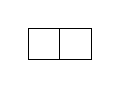
\begin{tikzpicture}[x=.4cm,y=.4cm]
    \begin{scope}
      \draw (0,0) rectangle (2,1);
      \draw (1,0) -- (1,1);
    \end{scope}
  \end{tikzpicture}~. Par contre, il existe deux triominos différents: un «~droit~» c'est-à-dire du type ~
  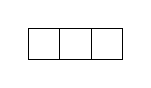
\begin{tikzpicture}[x=.4cm,y=.4cm]
    \begin{scope}
      \draw (0,1) rectangle (3,0);
      \draw (1,1) rectangle (2,0);
    \end{scope}
  \end{tikzpicture}~, et un «~coudé~» ~
  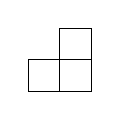
\begin{tikzpicture}[x=.4cm,y=.4cm]
    \begin{scope}
      \draw (0,1) rectangle (2,0);
      \draw (1,2) rectangle (2,0);
    \end{scope}
  \end{tikzpicture}~.
\begin{enumerate}
%\item Combien existe-il de tétrominos (assemblages de quatre carrés) ? % dépend si on compte le retournement : cinq ou bien sept. Généraliser ?
\item  On pose un monomino sur un coin d'un échiquier de taille $8\times 8$. Est-il possible de paver les $63=21\times 3$ cases restantes par des  triominos coudés ~~? 
  \item Même question en posant le monomino sur une case quelconque de l'échiquier.
  %\item Et avec des triominos droits ~~? % réserver pour le thème "invariants"
  \end{enumerate}
\begin{hint}
Penser aussi à des échiquiers de taille différente.
\end{hint}
\begin{sol}
% #généraliser puis prendre un cas particulier de l'énoncé général.
On montre plus généralement que c'est possible pour des échiquiers de taille $2^n$, par récurrence.
\end{sol}
\end{exo}

%%%%%%%%%%%%%%%%%
\begin{exo}[Régions délimitées par des droites]
 % Source : exo7 : 156

\begin{enumerate}
\item
Dans le plan, on consid\`ere trois droites $\Delta_{1},\Delta_{2},\Delta_{3}$ formant un
« vrai » triangle, autrement dit elles ne sont pas concourantes et il n'y en a pas deux parall\`eles.
Donner le nombre $R_{3}$ de r\'egions (zones blanches) d\'ecoup\'ees par ces trois droites.
\item
On consid\`ere quatre droites $\Delta_{1},\ldots,\Delta_{4}$, telles qu'il n'en existe pas
trois concourantes, ni deux parall\`eles. Donner le nombre $R_{4}$ de r\'egions d\'ecoup\'ees par
ces quatre droites.
\item
On consid\`ere $n$ droites $\Delta_{1},\ldots,\Delta_{n}$, telles qu'il n'en existe pas
trois concourantes, ni deux parall\`eles. Soit $R_{n}$ le nombre de r\'egions d\'elimit\'ees par
$\Delta_{1}\ldots\Delta_{n}$, et $R_{n-1}$ le nombre de r\'egions d\'elimit\'ees par
$\Delta_{1}\ldots\Delta_{n-1}$. Montrer que $R_{n}=R_{n-1}+n$.
\item
Calculer par r\'ecurrence le nombre de r\'egions d\'elimit\'ees par $n$ droites en position
g\'en\'erale, c'est-\`a-dire telles qu'il n'en existe pas trois concourantes ni deux parall\`eles.
\end{enumerate}

\begin{sol}
Montrons par r\'ecurrence sur $n \geqslant 1$ la proposition suivante :
$$\mathcal{H}_n :  \quad n \text{\  droites en position g\'en\'erale d\'ecoupent le plan en \ } R_n = \frac{n(n+1)}{2}+1
\text{\  r\'egions.}$$

\begin{itemize}
\item[$\bullet$] pour $n=1$ alors une droite divise le plan en deux r\'egions. $\mathcal{H}_1$ est vraie.

\item[$\bullet$] Soit $n\geqslant 2$ et supposons que $\mathcal{H}_{n-1}$ soit vraie, et montrons $\mathcal{H}_n$.
Soient $\Delta_1,\ldots,\Delta_n$ $n$ droites en position
g\'en\'erale, la droite $\Delta_n$ rencontre les droites
$\Delta_1,\ldots,\Delta_{n-1}$ en $n-1$ points, donc $\Delta_n$
traverse (et d\'ecoupe en deux) $n$ r\'egions du d\'ecoupage
$\Delta_1,\ldots,\Delta_{n-1}$. Le d\'ecoupage par $\Delta_n$
donne donc la relation $R_n=R_{n-1}+n$.

Or par hypoth\`ese de r\'ecurrence $\mathcal{H}_{n-1}$ : $R_{n-1}
= \frac{(n-1)n}{2}+1$ donc
$$  R_n = R_{n-1}+n =  \frac{(n-1)n}{2}+1+n=\frac{n(n+1)}{2}+1 $$
Et $\mathcal{H}_n$ est vraie.\\
Ainsi $\forall n\in\N^* \quad \mathcal{H}_{n-1}\Rightarrow
\mathcal{H}_{n}$.

\item[$\bullet$] Conclusion :  par r\'ecurrence on a montr\'e que $\mathcal{H}_n$ est vraie quelque soit $n \geqslant 1$.

\end{itemize}
\end{sol}
\end{exo}








%%%%%%%%%%%%%%%%%
\begin{exo}[Une erreur de raisonnement]
La \og preuve\fg{} suivante prétend montrer par récurrence sur $n \geq 1$ qu'étant donné $n$ nombres réels $u_1, u_2, \ldots, u_n \in \R$, ils sont en fait tous égaux.

\begin{quote}
  \textbf{Initialisation.} S'il n'y a qu'un nombre $u_1$, il n'y a rien à montrer.

  \textbf{Hérédité.} Soit $n \geq 1$ un entier tel que $n$ nombres réels soient toujours égaux et donnons-nous $(n+1)$ nombres réels $u_1, u_2, \ldots, u_n, u_{n+1} \in \R$.

  D'après l'hypothèse de récurrence, on a d'une part $u_{1} = u_{2} = \cdots = u_{n}$ et d'autre part $u_{2} = \cdots = u_{n} = u_{n+1}$. Cela entraîne que $u_{1} = u_{2} = \cdots = u_{n} = u_{n+1}$, et montre donc la propriété voulue.
\end{quote}

Le résultat est évidemment faux. Où se trouve  l'erreur de raisonnement ?
\begin{sol}
La preuve de l'hérédité n'est correcte que pour $n\geq 2$, pas $n\geq 1$ si on regarde attentivement.
\end{sol}
\end{exo}





%%%%%%%%%%%%%%%%%
\begin{exo}[Tour d'Hanoï]
% source Maxime ex 7313
La \emph{tour d'Hanoï} est un jeu à un joueur qui se joue comme suit~: on dispose de trois piquets et de $n$ disques percés de tailles différentes. Une position légale du jeu est une disposition des $n$ disques sur les piquets qui soit telle que sur chaque piquet, un disque n'est jamais posé sur un autre disque plus petit. Dans la position de départ, tous les disques sont sur le premier piquet. Le but du jeu est d'arriver à la situation où tous les disques sont sur le troisième piquet, en ne déplaçant qu'un disque à la fois (on n'a évidemment accès qu'au disque le plus haut de chaque piquet) et en ne passant que par des positions légales.
\begin{center}
  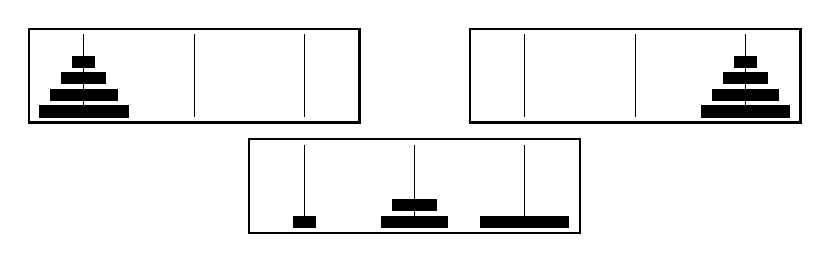
\begin{tikzpicture}[x=1.4cm,y=.7cm]
    \begin{scope}
      \draw[thick] (0,-.1) rectangle (3,1.6);
      \draw (.5,0)--(.5,1.5);
      \draw (1.5,0)--(1.5,1.5);
      \draw (2.5,0)--(2.5,1.5);
      \draw[fill=black] (.1,0) rectangle (.9,.2);
      \draw[fill=black] (.2,.3) rectangle (.8,.5);
      \draw[fill=black] (.3,.6) rectangle (.7,.8);
      \draw[fill=black] (.4,.9) rectangle (.6,1.1);
    \end{scope}
    
%    \draw[thick, ->] (3.3,.75)--(3.7,.75);
    
    \begin{scope}[shift={+(4,0)}]
      \draw[thick] (0,-.1) rectangle (3,1.6);
      \draw (.5,0)--(.5,1.5);
      \draw (1.5,0)--(1.5,1.5);
      \draw (2.5,0)--(2.5,1.5);
      \draw[fill=black] (2.1,0) rectangle (2.9,.2);
      \draw[fill=black] (2.2,.3) rectangle (2.8,.5);
      \draw[fill=black] (2.3,.6) rectangle (2.7,.8);
      \draw[fill=black] (2.4,.9) rectangle (2.6,1.1);
    \end{scope}

    \begin{scope}[shift={+(4,0)}]
      \draw[thick] (0,-.1) rectangle (3,1.6);
      \draw (.5,0)--(.5,1.5);
      \draw (1.5,0)--(1.5,1.5);
      \draw (2.5,0)--(2.5,1.5);
      \draw[fill=black] (2.1,0) rectangle (2.9,.2);
      \draw[fill=black] (2.2,.3) rectangle (2.8,.5);
      \draw[fill=black] (2.3,.6) rectangle (2.7,.8);
      \draw[fill=black] (2.4,.9) rectangle (2.6,1.1);
    \end{scope}

%    \draw [thick, ->] (1,-.3) to [out=-90, in=180] (1.8,-1.25);
%    \draw [thick, ->] (5.2,-1.25) to [out=0, in=-90] (6,-.3);

    
        \begin{scope}[shift={+(2,-2)}]
      \draw[thick] (0,-.1) rectangle (3,1.6);
      \draw (.5,0)--(.5,1.5);
      \draw (1.5,0)--(1.5,1.5);
      \draw (2.5,0)--(2.5,1.5);
      \draw[fill=black] (1.2,0) rectangle (1.8,.2);
      \draw[fill=black] (1.3,.3) rectangle (1.7,.5);
      \draw[fill=black] (2.1,0) rectangle (2.9,.2);
      \draw[fill=black] (.4,0) rectangle (.6,.2);
    \end{scope}
      \end{tikzpicture}\\
Positions initiale, finale et intermédiaire
\end{center}
\begin{enumerate}
\item Montrer que quel que soit $n$, le jeu de la tour d'Hanoï est résoluble.
\item Quel est le nombre minimum de coups nécessaires pour le résoudre~?
\end{enumerate}
\end{exo}

%%%%%%%%%%%%%%%%%
%%%%%%%%%%%%%%%%%
\begin{exo}[Deux résultats sur les tournois]
% Source: Maxime ex 2141

Dans un \emph{tournoi d'ordre $n$} (au sens mathématique), $n \geq 2$ équipes s'affrontent une fois chacune. Chaque match désigne un vainqueur (il n'y a donc pas de match nul).
\begin{enumerate}
\item Montrer que quelle que soit l'issue du tournoi, il sera possible de numéroter les équipes $\acute E_1$, $\acute E_2$, $\ldots$, $\acute E_n$ de telle sorte que, pour tout $1 \leq i < n$, l'équipe $\acute E_i$ ait battu l'équipe $\acute E_{i+1}$ \emph{(théorème de Rédei, 1934)}.
\item Un tournoi est dit \emph{équilibré} si chaque équipe a gagné autant de matchs qu'elle en a perdu. Montrer qu'il existe un tournoi équilibré d'ordre $n$ si et seulement si $n$ est impair.
  \end{enumerate}
\begin{hint}
\begin{enumerate}
\item 
\item Penser à la récurrence
\end{enumerate}
\end{hint}
\begin{sol}
\begin{enumerate}
\item Montrons le résultat par récurrence sur $n$ le nombre d'équipes.\\
\textbf{Initialisation.} Pour deux équipes, c'est clair.\\
\textbf{Hérédité.} Soit $n\in \N$ et supposons qu'on sache ordonner $n$ équipes comme indiqué. Quitte à renuméroter les équipes, supposons qu'on ait le classement suivant des équipes $\acute E_1,\ldots,\acute
E_n$ : $\acute E_1 > \acute E_2 > \ldots > \acute E_n$, où A > B signifie que A a battu B. Il s'agit d'insérer l'équipe $\acute E_{n+1}$ dans ce classement. Si elle a gagné contre $\acute E_1$, on l'insère en première position. Sinon, on continue : si elle a gagné contre $\acute E_2$, on l'insère en 2e position etc. Si elle a perdu contre $\acute E_n$ (et donc contre tout le monde), on l'insère en dernière position.\\
\textbf{Conclusion.} D'après le principe de récurrence, on a montré que pour n'importe quel nombre $n$ d'équipes, on peut établir un tel classement.\\
\item “$\Rightarrow$)” Si le tournoi est équilibré, chaque équipe a autant de victoires que de défaites et donc a joué un nombre pair de matchs. Chaque équipe joue $n-1$ matchs, ainsi $n$ est impair.\\
“$\Leftarrow$)” Par récurrence sur le nombre d'équipes.
% à faire
\end{enumerate}
\end{sol}
\end{exo}



%%%%%%%%%%%%%%%%%
\begin{exo}[Héréditaire ? Vraie ?]
Pour tout $n \in \N$, on note $A(n)$ l'assertion \og $2n+1 \leq 2^n$.\fg

La propriété $A(n)$ est-elle héréditaire? Est-elle vraie pour tout entier $n$ ? Pour certains $n$ ?

\begin{hint}
On peut tester à la main pour des petites valeurs de $n$.
\end{hint}
\begin{sol}
Pour tout $n \in \N$, on note $A(n)$ l'assertion \og $2n+1 \leq 2^n$.\fg Montrons que cette assertion est héréditaire.\\ 
\textbf{Hérédité.} Soit $n \geq 1$, on suppose que $A(n)$ est vraie. On a : 
$$2n+1 \leq 2^n \Leftrightarrow 2(2n+1) \leq 2^{n+1}.$$
Par ailleurs, $2(n+1)+1 \leq 2(2n+1) \Leftrightarrow 1 \leq 2n$, ce qui est vrai pour tout $n \geq 1$.
Ainsi $A(n+1)$ est vraie.\\
On remarque que $A(0)$ est vraie, cependant on ne peut y appliquer l'hérédité. $A(1)$ et $A(2)$ sont fausses mais $A(3)$ est vraie. \\
\textbf{Conclusion.} On peut donc conclure à l'aide de l'hérédité, que pour tout $n \geq 3$, $A(n)$ est vraie.
\end{sol}
\end{exo}





%%%%%%%%%%%%%%%%%
\begin{exo}[Coloriage]
% Source : Animath / Cécile Gachet
\begin{multicols}{2}
\null \vfill
Soit $n\geq 1$ un entier. On trace $n$ cercles dans le plan.

Montrer qu'on peut colorier chaque région du plan ainsi délimitée avec exactement deux couleurs (bleu et rouge par exemple) de manière à ce que deux régions séparées par un arc de cercle soient toujours de couleur différente.
\vfill \null    
\columnbreak
\begin{center}
\begin{tikzpicture}[line cap=round,line join=round,>=triangle 45,x=1.0cm,y=1.0cm,scale=0.8]
\clip(-3.60736,0.2966) rectangle (2.38214,5.70046);
\draw(-1.58,3.44) circle (1.6595180023127198cm);
\draw(0.16,3.24) circle (1.9016834647227705cm);
\draw(-1.5,1.68) circle (1.0539987928599734cm);
\draw(0.64,4.3) circle (1.0001999800039991cm);
\end{tikzpicture}
\end{center}
\end{multicols}
\begin{sol}
Pour tout $n\in \N$, notons $P(n)$ l'assertion \og  étant donnés $n$ cercles du plan, on peut colorier chaque région du plan ainsi délimitée avec exactement deux couleurs (bleu et rouge par exemple) de manière à ce que deux régions séparées par un arc de cercle soient toujours de couleur différente.\fg

Montrons que pour tout $n\in \N$, l'assertion $P(n)$ est vraie, par récurrence sur $n$.

\noindent \textbf{Initialisation.} Pour $n=0$, c'est-à-dire lorsqu'il n'y a aucun cercle, c'est évident.

\noindent \textbf{Hérédité.} Soit $n\in N$ tel que $P(n)$ soit vraie. Montrons $P(n+1)$. Soit donc $\mathcal C_1$, ... $\mathcal C_{n+1}$ des cercles du plan. En enlevant provisoirement le dernier cercle, on a donc $n$ cercles, et d'après l'hypothèse de récurrence, on peut colorier chaque région du plan ainsi délimitée en bleu et rouge de manière à ce que deux régions séparées par un arc de cercle soient toujours de couleur différente.

Rajoutons alors le $(n+1)$-ème cercle. Il croise certaines régions coloriées et la propriété demandée tombe alors en défaut. On peut alors inverser le coloriage des régions qui sont à l'intérieur de $\mathcal C_{n+1}$, ce qui donne un nouveau coloriage. Montrons qu'il satisfait à la condition de l'énoncé. Il s'agit de vérifier que pour tout arc de cercle délimitant deux régions, les couleurs de part et d'autre sont différentes. S'il s'agit d'un arc qui appartient aux $n$ premiers cercles, les couleurs étaient différentes lors du premier coloriage. Si l'arc est à l'extérieur de $\mathcal C_{n+1}$, les couleurs n'ont pas changé, et sinon, elles ont été inversées donc sont différentes. Si par contre l'arc appartient au dernier cercle $\mathcal C_{n+1}$, alors les deux couleurs étaient identiques avant de changer le coloriage, et elles sont maintenant distinctes puisque la couleur à l'intérieur de $\mathcal C_{n+1}$ a été changée.

Finalement, $P(n+1)$ est vraie, ce qui conclut le raisonnement.
\end{sol}
\end{exo}

% autre exo : régions dans un cercle coupées par des droites, voir Gowers : 2, 4, 8, 16..., 31 !


%%%%%%%%%%%%%%%%%
\begin{exo}[Erreur de raisonnement, bis]
% SOurce : Maxime
La «~preuve~» suivante prétend montrer par récurrence que tous les entiers supérieurs ou égaux à deux sont pairs.

\begin{quote}
  \textbf{Initialisation.} L'entier $2$ est bien pair.

  \textbf{Hérédité.} Soit $n>2$ un entier. Écrivons $n$ comme la somme de deux entiers strictement inférieurs : $n=a+b$. Par hypothèse de récurrence, $a$ et $b$ sont pairs. Donc $a+b$ est également pair.
\end{quote}

Le résultat est évidemment faux. Où se trouve  l'erreur de raisonnement~?
\begin{sol}
Les entiers $a$ et $b$ ne sont pas forcément $\geq 2$...
\end{sol}
\end{exo}




